\section{Overall Pipeline}

The complete workflow starts from Direct Numerical Simulation density fields,
applies preprocessing and physically motivated data augmentation, trains a
generative diffusion model, and evaluates generated samples against validation
data. Figure~\ref{fig:diffusion_pipeline} gives the general principle of this
surrogate modeling approach.

\begin{figure}[H]
\centering
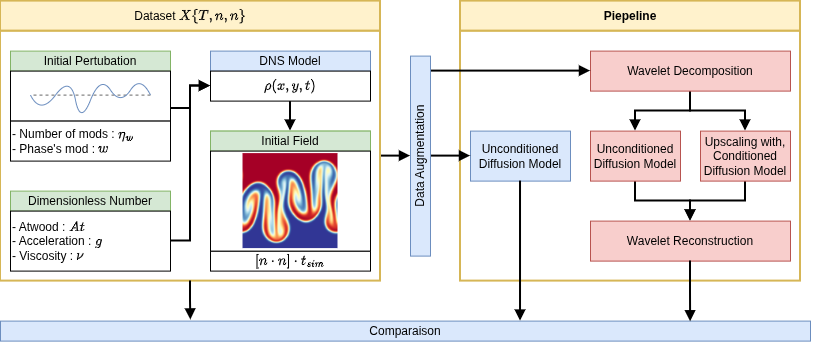
\includegraphics[width=0.95\textwidth]{figures/intro/pipeline.png}
\caption{General principle of the diffusion-based surrogate modeling approach used in this work.}
\label{fig:diffusion_pipeline}
\end{figure}

